\documentclass[9pt,a4paper]{article}
\usepackage[utf8]{inputenc}
\usepackage{amsmath}
\usepackage{amsfonts}
\usepackage{amssymb}
\usepackage{makeidx}
\usepackage{alltt}
\usepackage{booktabs}
\usepackage[dvips]{graphicx}


\author{Wang Feng \\ wang\_feng@live.com}
\title{a 2D TM FDTD Solver}
\begin{document}

\maketitle

\section{a Short Introduction}

I coded this solver following Dennis M. Sullivan's textbook \textit{Electromagnetic Simulation Using the FDTD Method}, 
and tested the code under Linux x86\_64 with g++4.6 successfully. 

This solver simulates a plane wave interacting with a circular cylinder, which is a perfectly electrical conductor.   
The simulation field is 100X100, the center of the cylinder locates at (50, 50), and the radius is set to 10. 
The width of the incoming wave is set to 15. And all the parameters configuration can be found within file src/fdtd.cpp.

\section{Simulation Result}

The current on the surface of the cylinder in both illuminated and shadowed sited could be found in Figure \ref{pic:vs}, which is quite
similar to the MOT result.


\begin{figure}
\centering
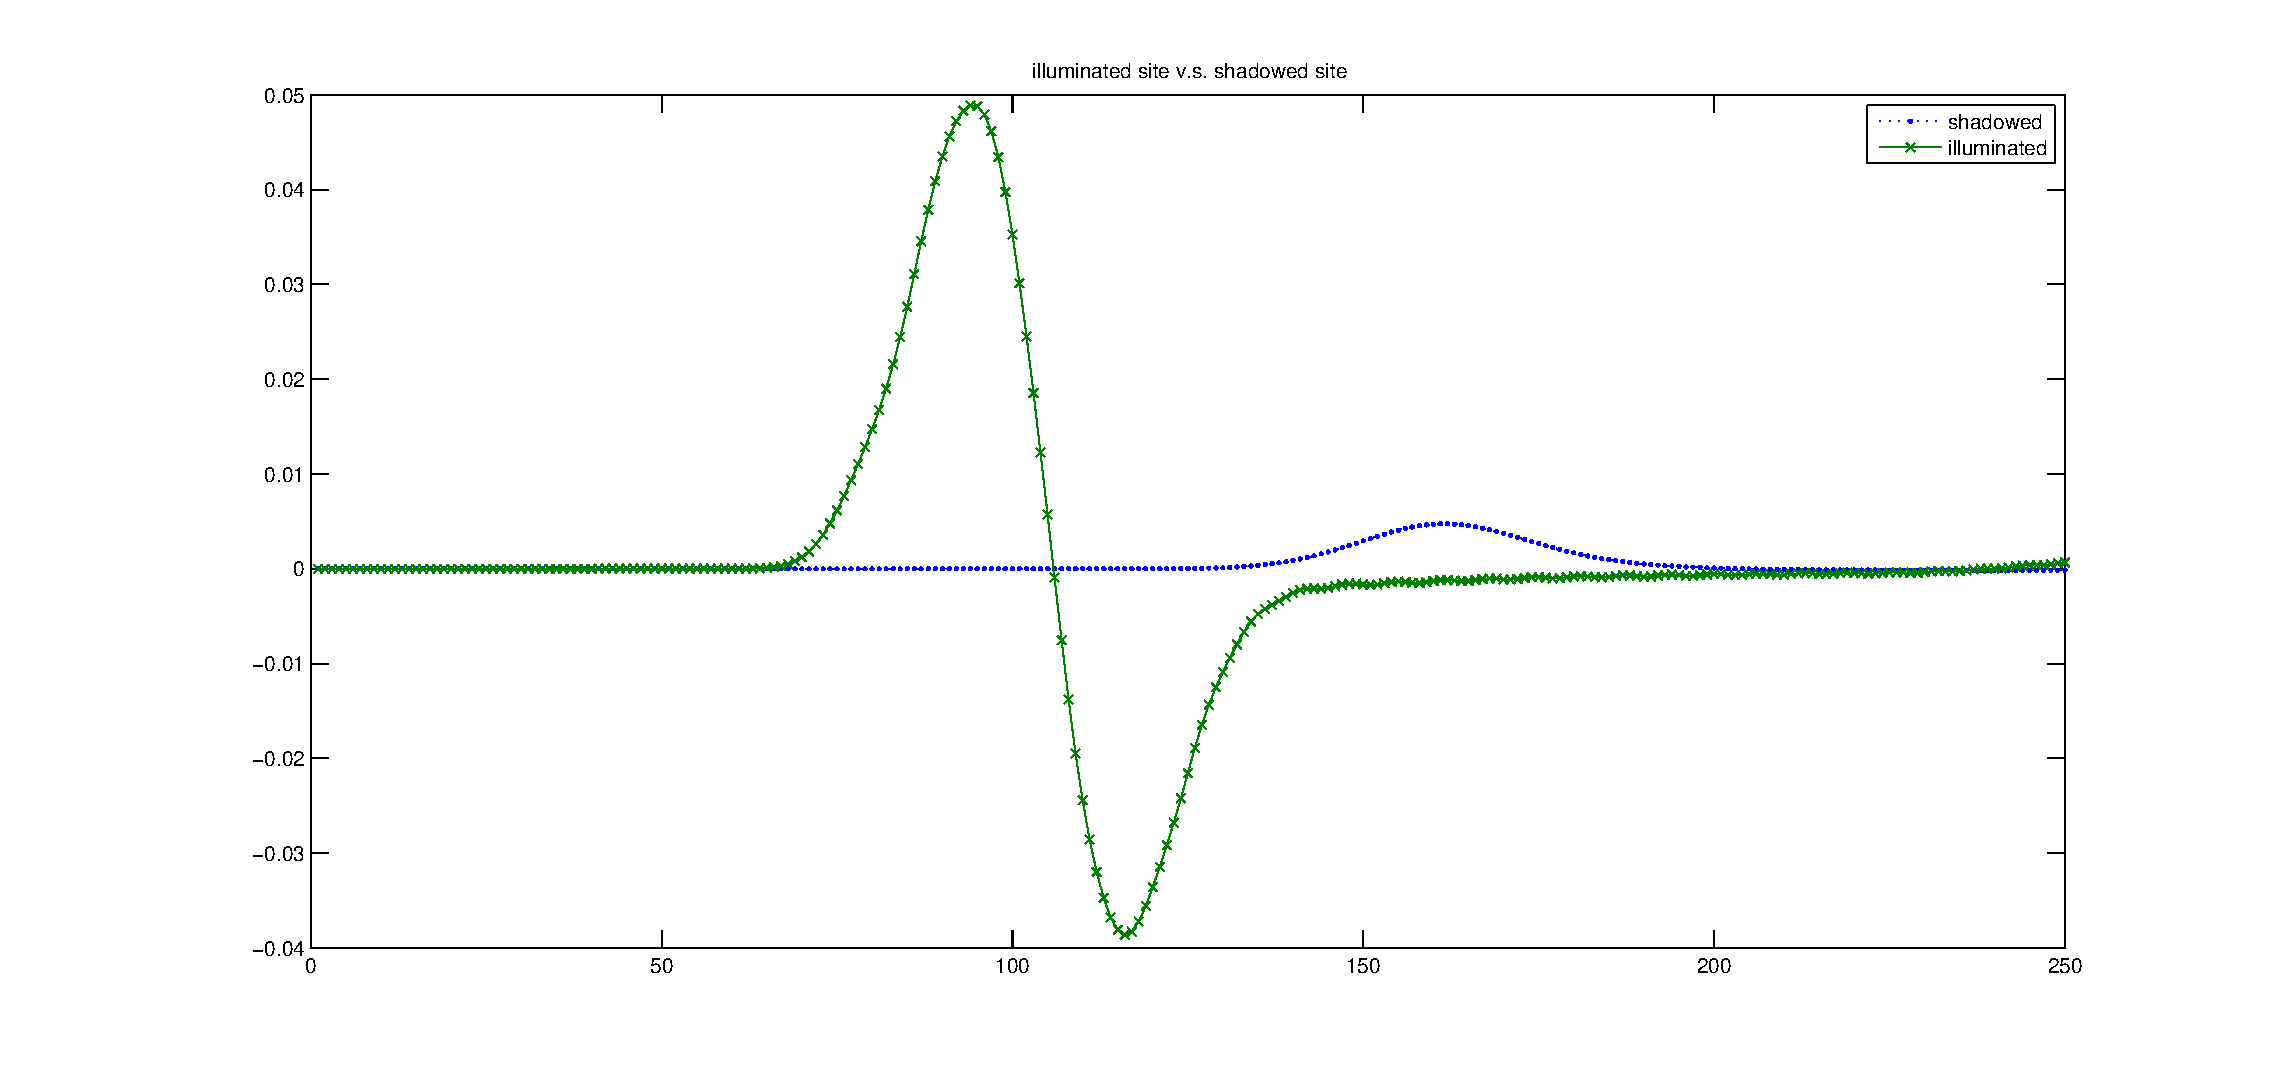
\includegraphics[angle=270,
    width=0.8\textwidth]{ill.vs.sh.eps}
\caption{The current on the surface of the scatter in both the shadowed and illuminated face, when the incoming wave pulse width is 15.}
\label{pic:vs}
\end{figure}

The simulation of $E_z$ could be directly perceived from Figure \ref{pic:ez80} to Figure \ref{pic:ez200}.


\begin{figure}
\centering
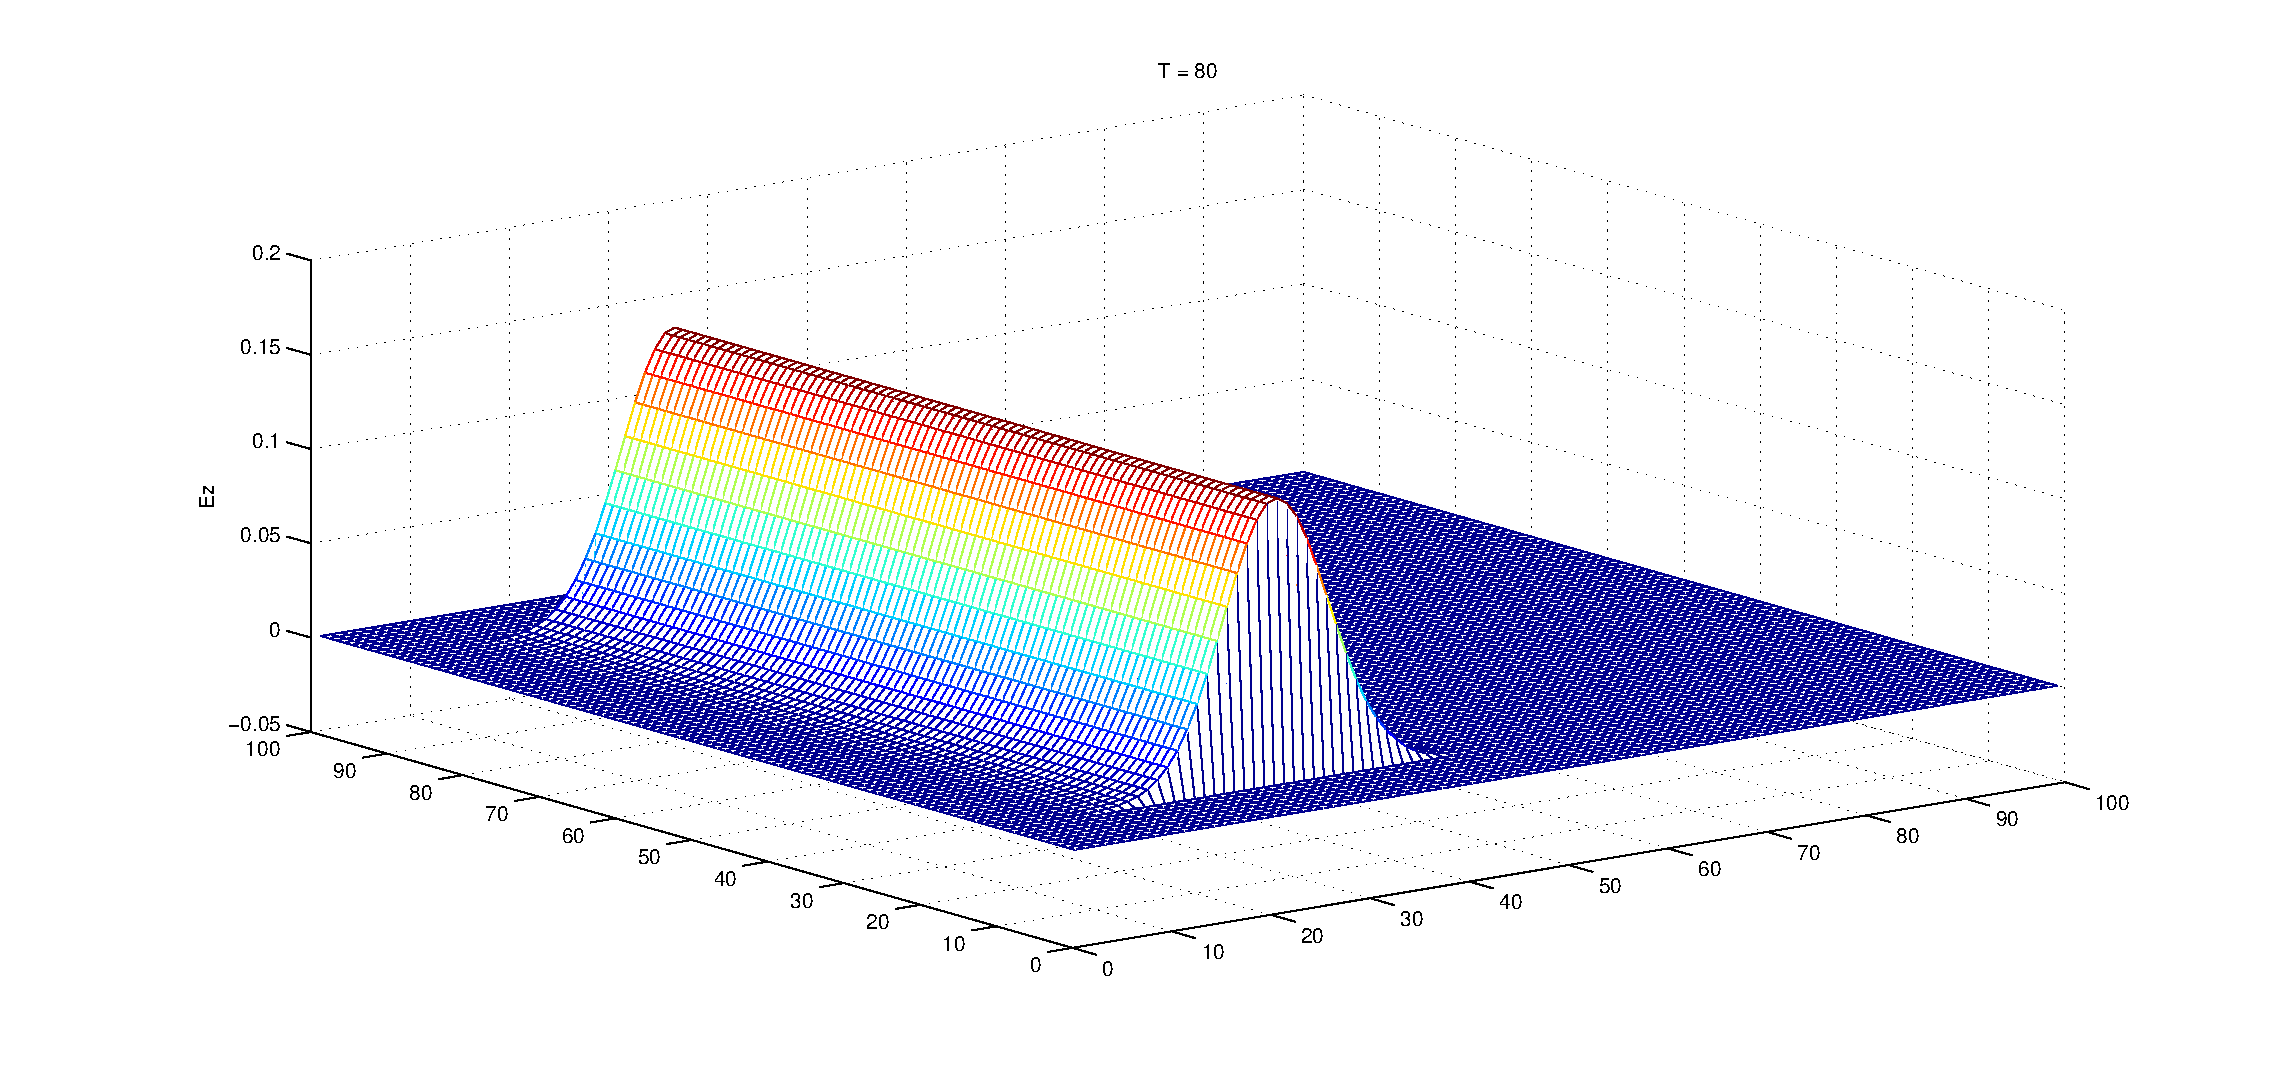
\includegraphics[angle=90,
    width=0.8\textwidth]{ez.80.eps}
\caption{$E_z$ when T = 80.}
\label{pic:ez80}
\end{figure}

\begin{figure}
\centering
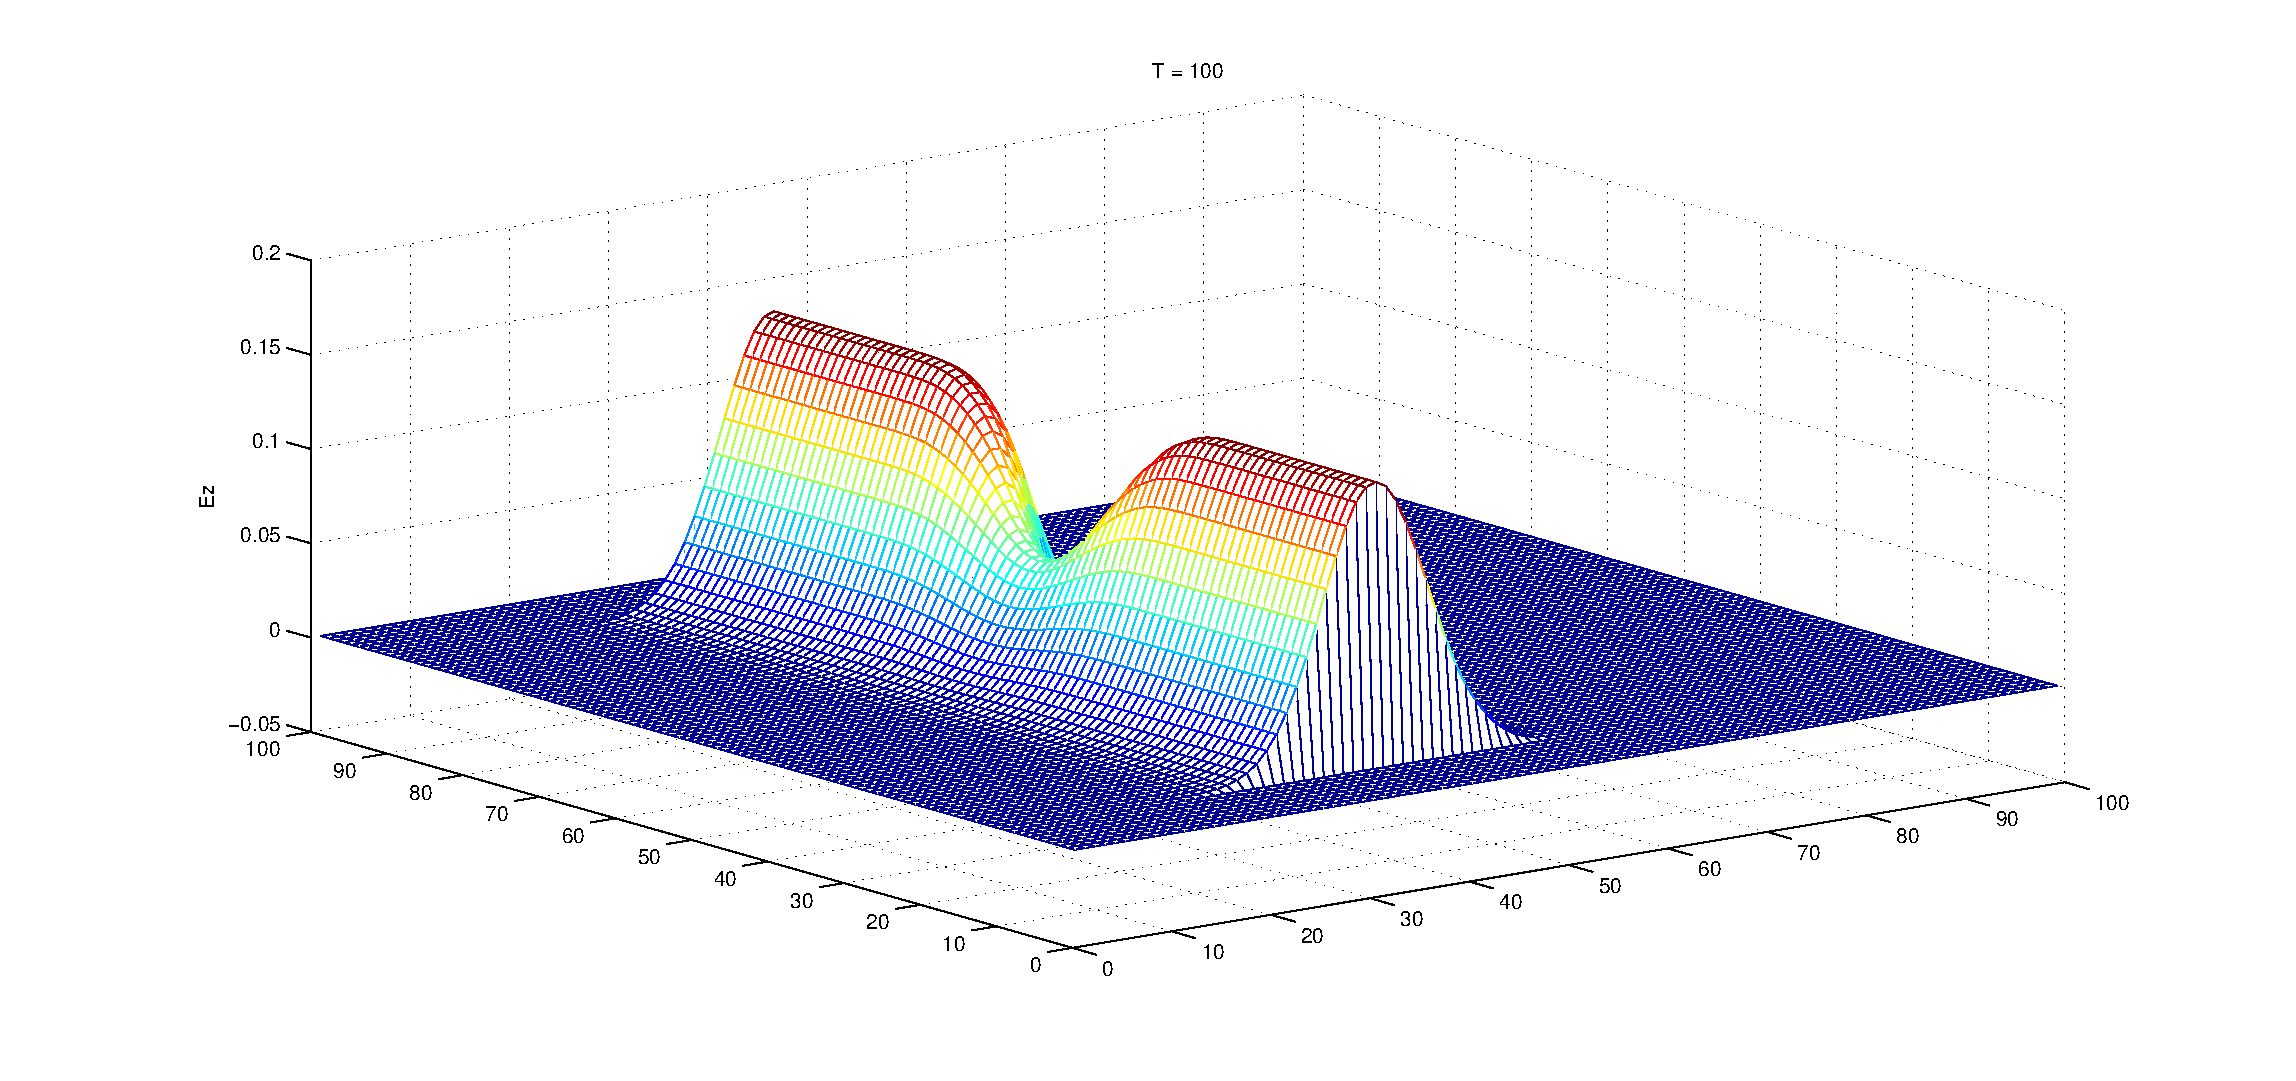
\includegraphics[angle=270,
    width=0.8\textwidth]{ez.100.eps}
\caption{$E_z$ when T = 100.}
\label{pic:ez100}
\end{figure}

\begin{figure}
\centering
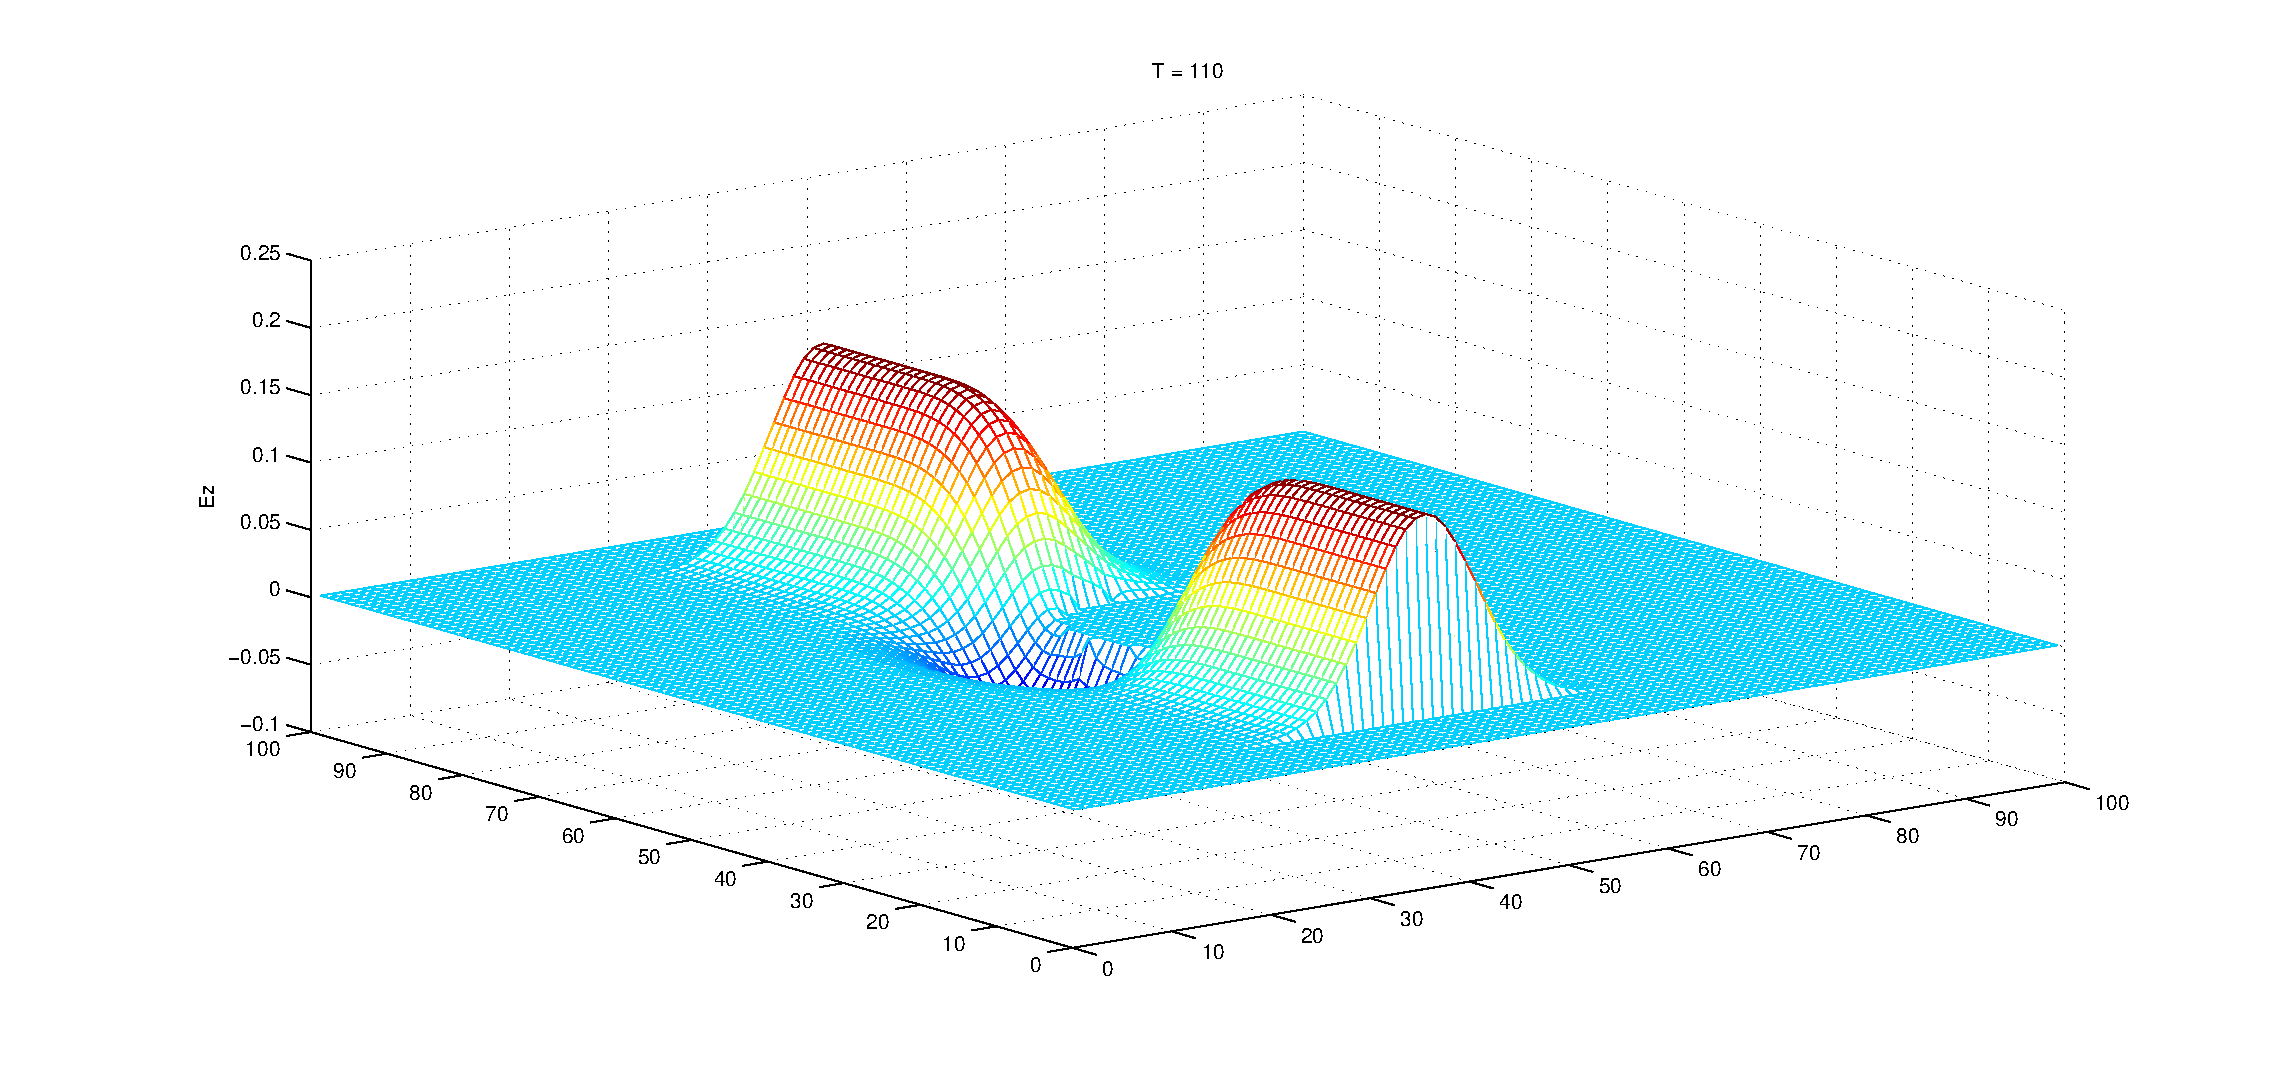
\includegraphics[angle=270,
    width=0.8\textwidth]{ez.110.eps}
\caption{$E_z$ when T = 110.}
\label{pic:ez110}
\end{figure}

\begin{figure}
\centering
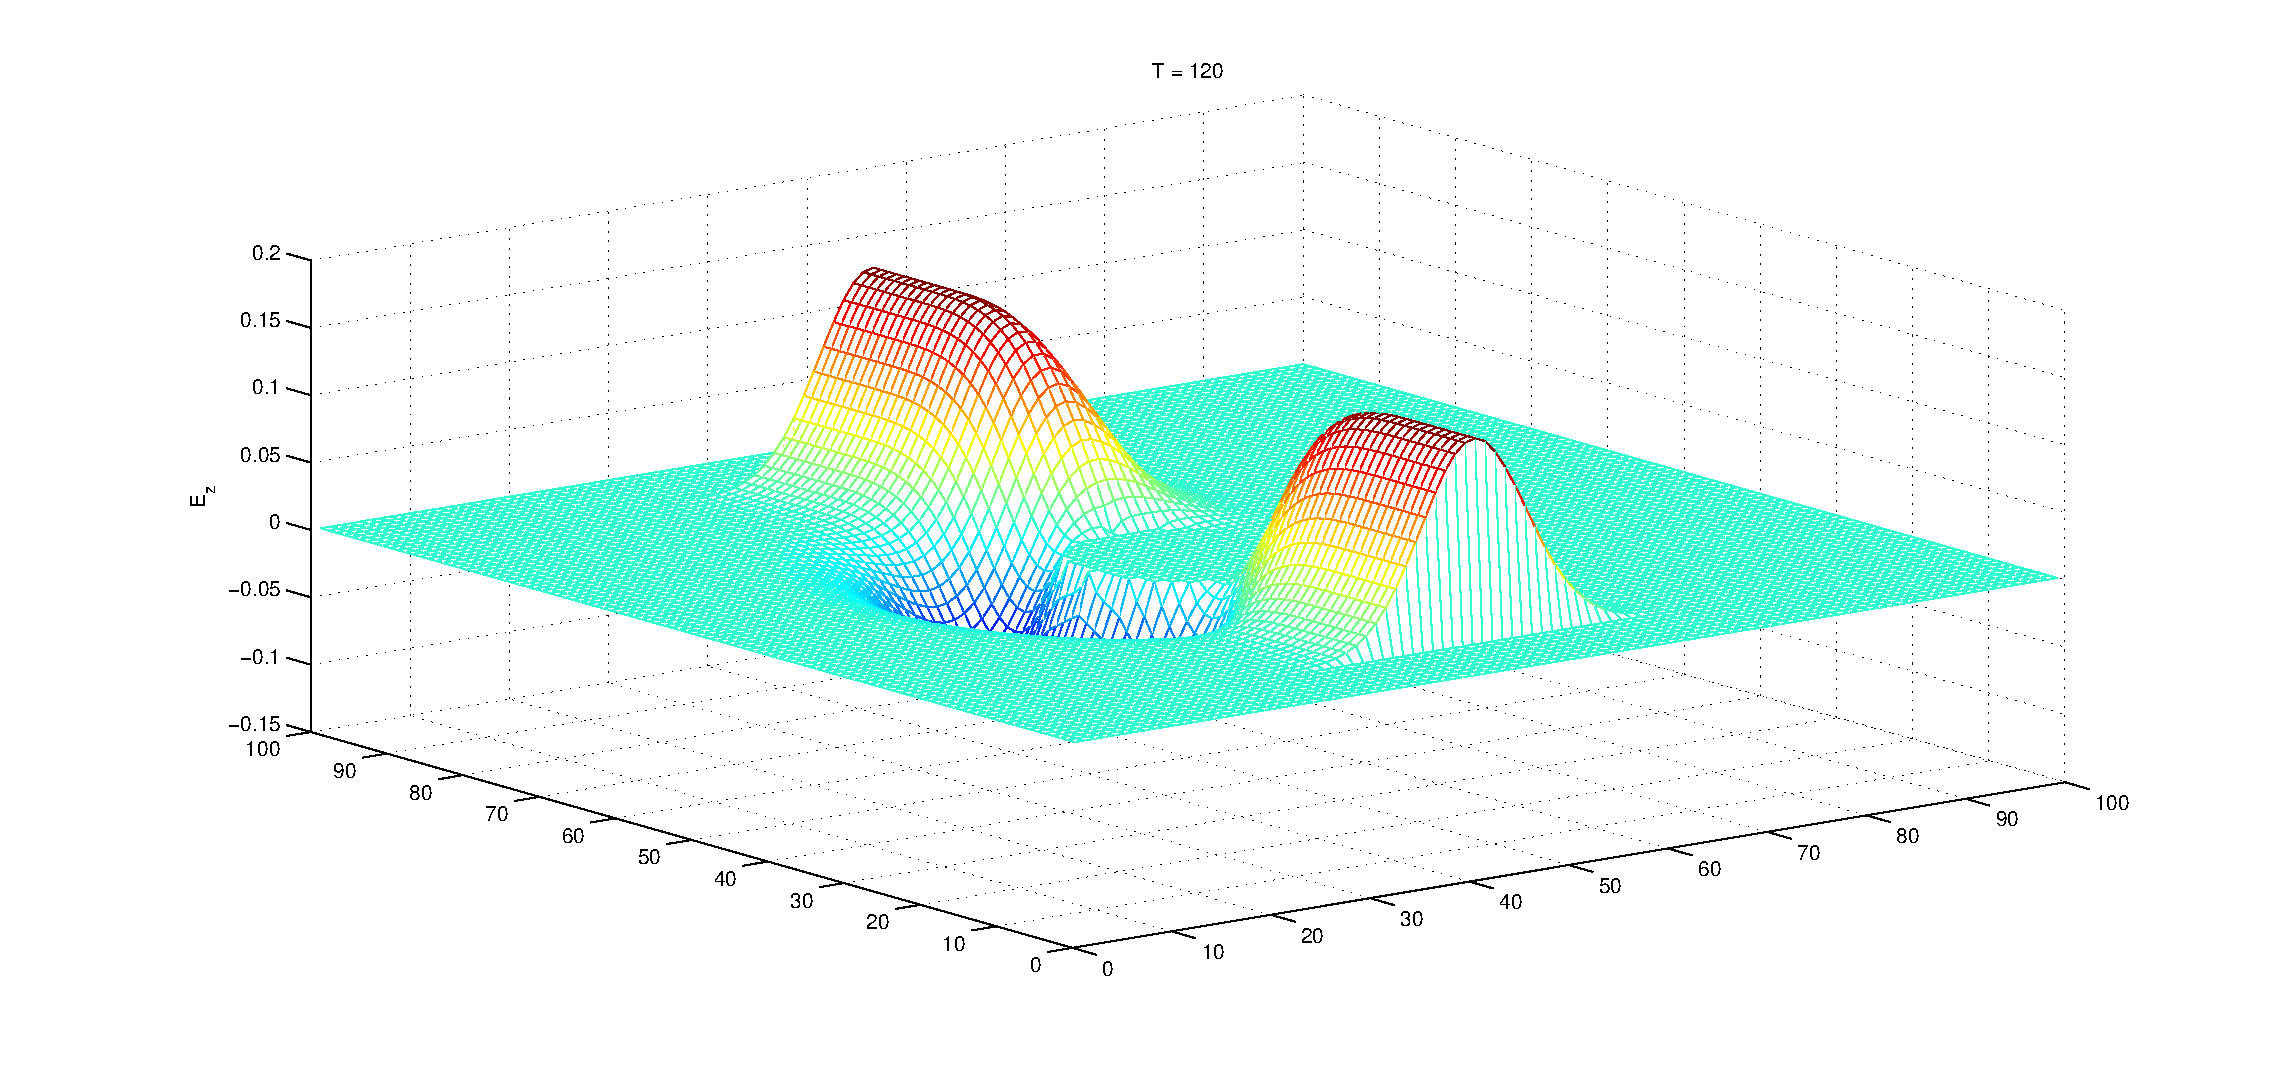
\includegraphics[angle=270,
    width=0.8\textwidth]{ez.120.eps}
\caption{$E_z$ when T = 120.}
\label{pic:ez120}
\end{figure}

\begin{figure}
\centering
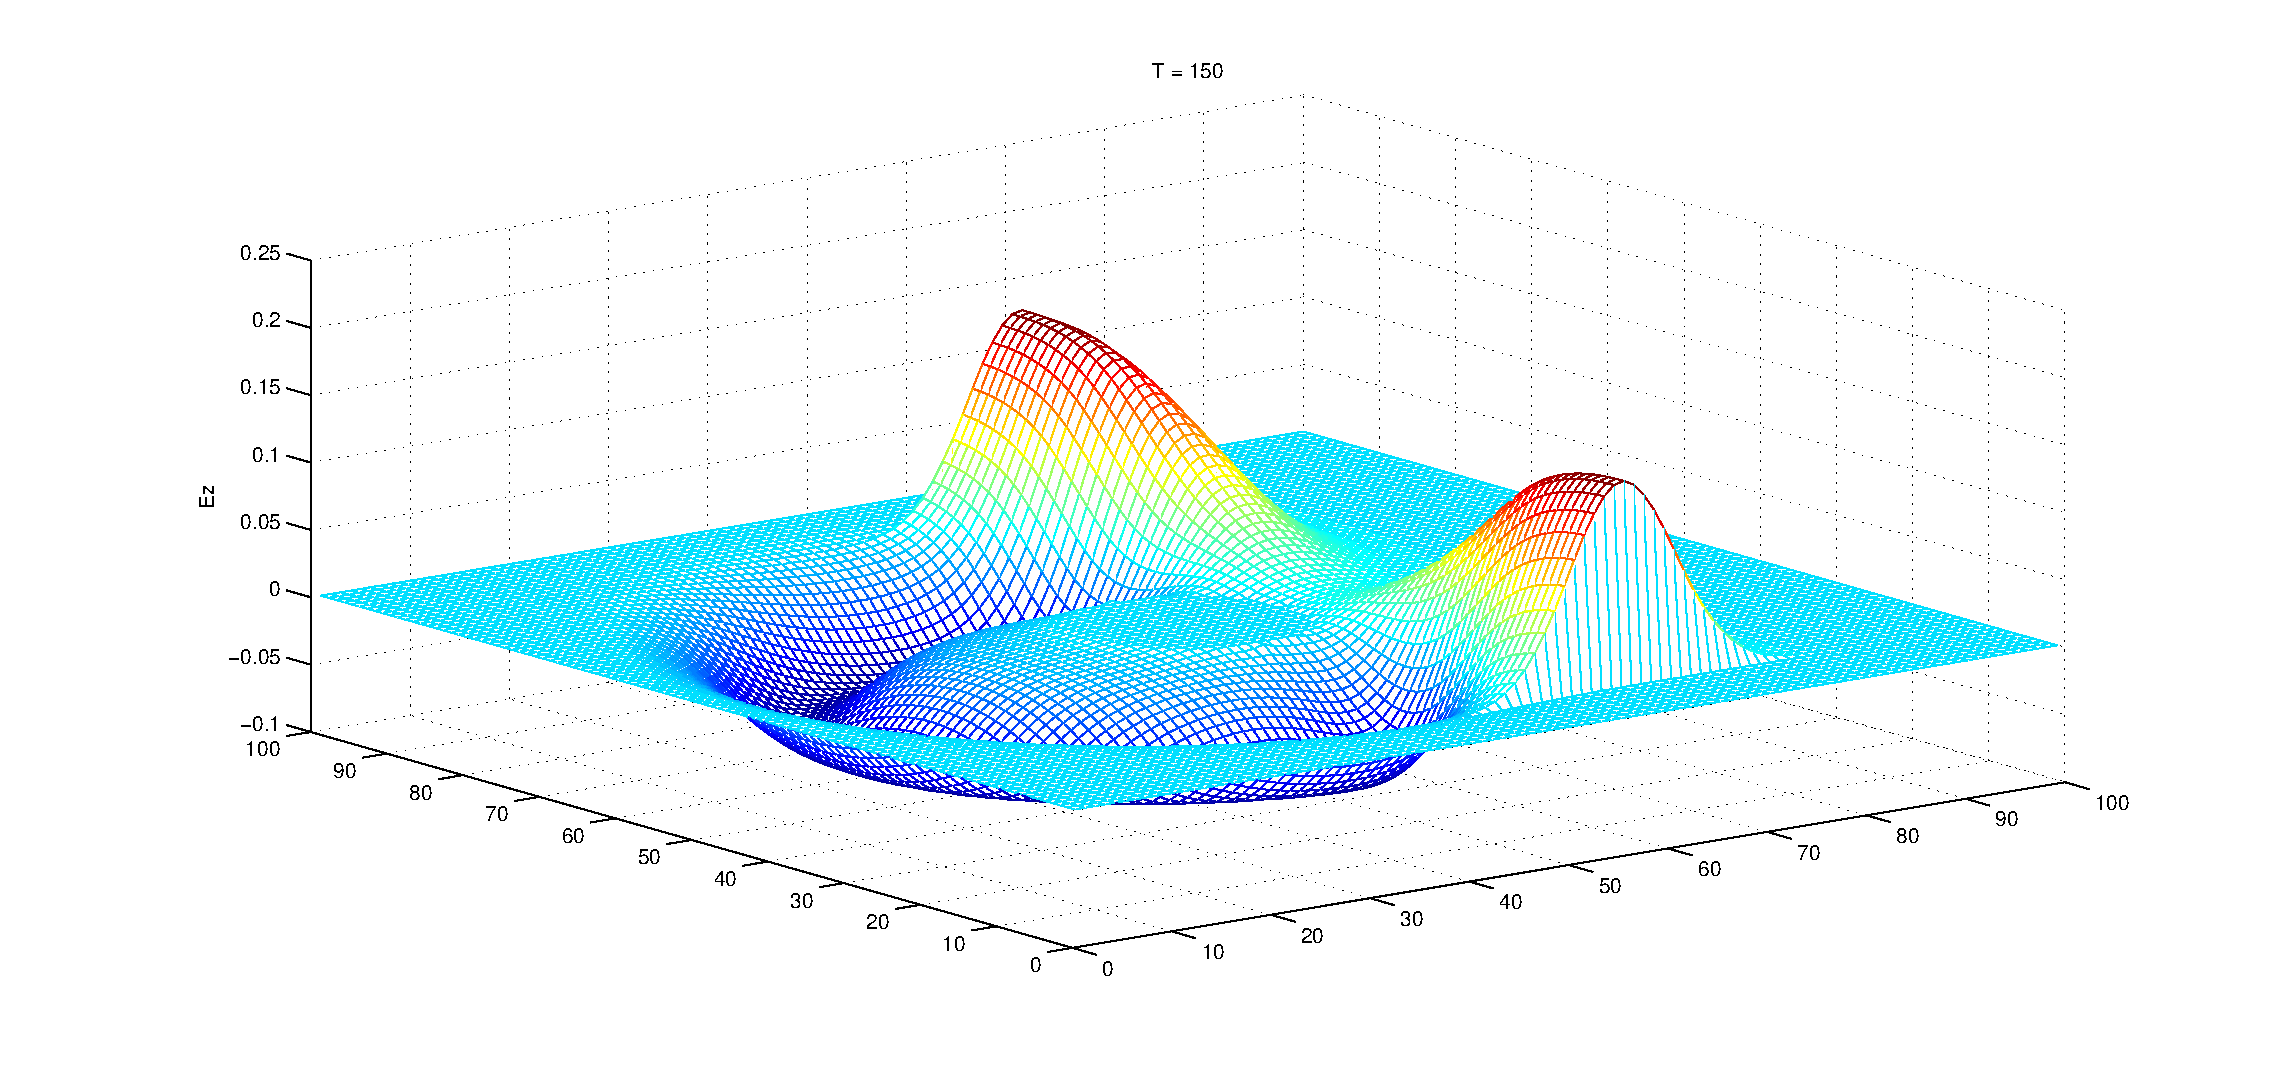
\includegraphics[angle=270,
    width=0.8\textwidth]{ez.150.eps}
\caption{$E_z$ when T = 150.}
\label{pic:ez150}
\end{figure}

\begin{figure}
\centering
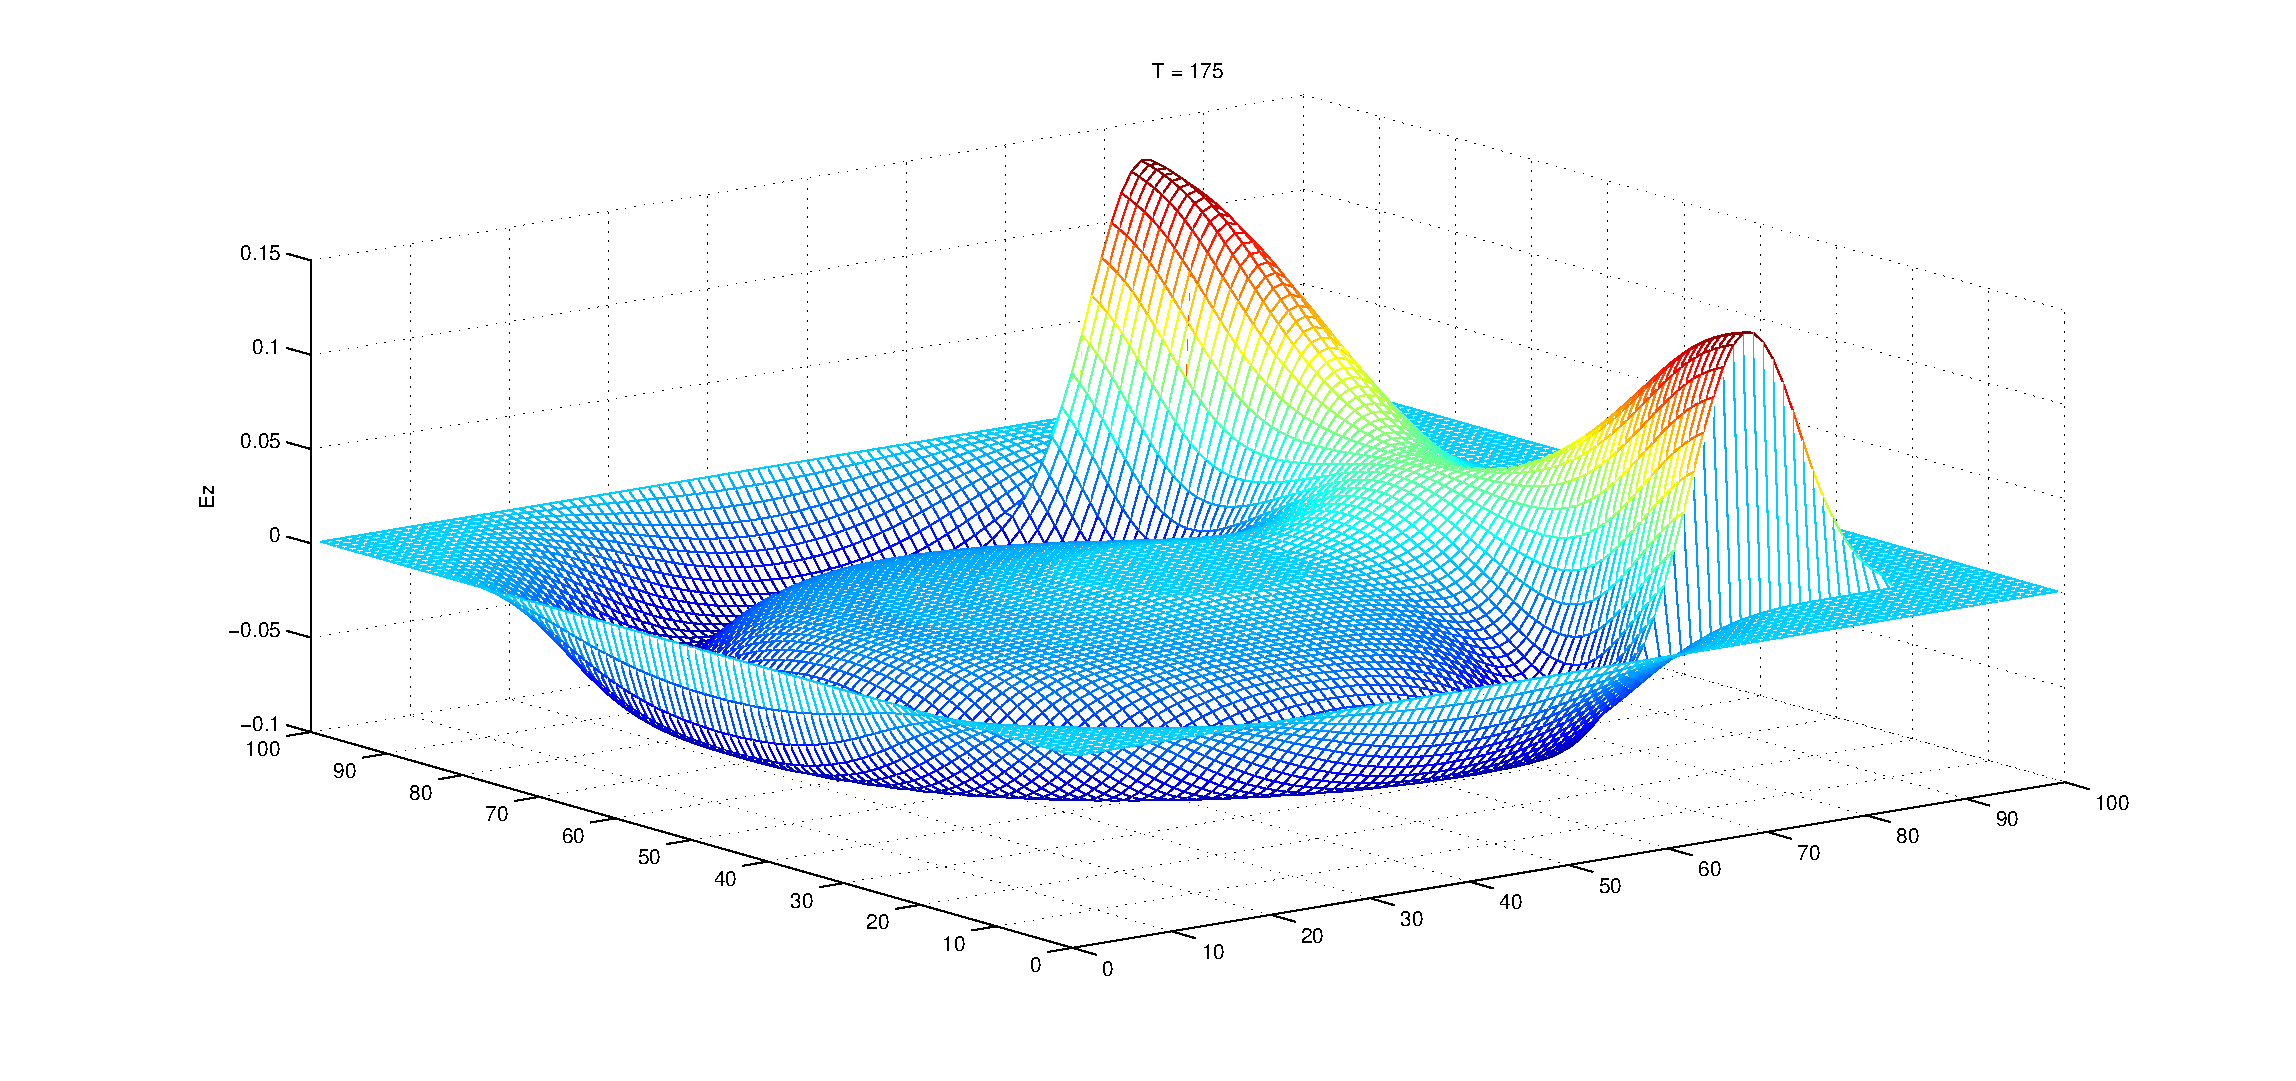
\includegraphics[angle=270,
    width=0.8\textwidth]{ez.175.eps}
\caption{$E_z$ when T = 175.}
\label{pic:ez175}
\end{figure}

\begin{figure}
\centering
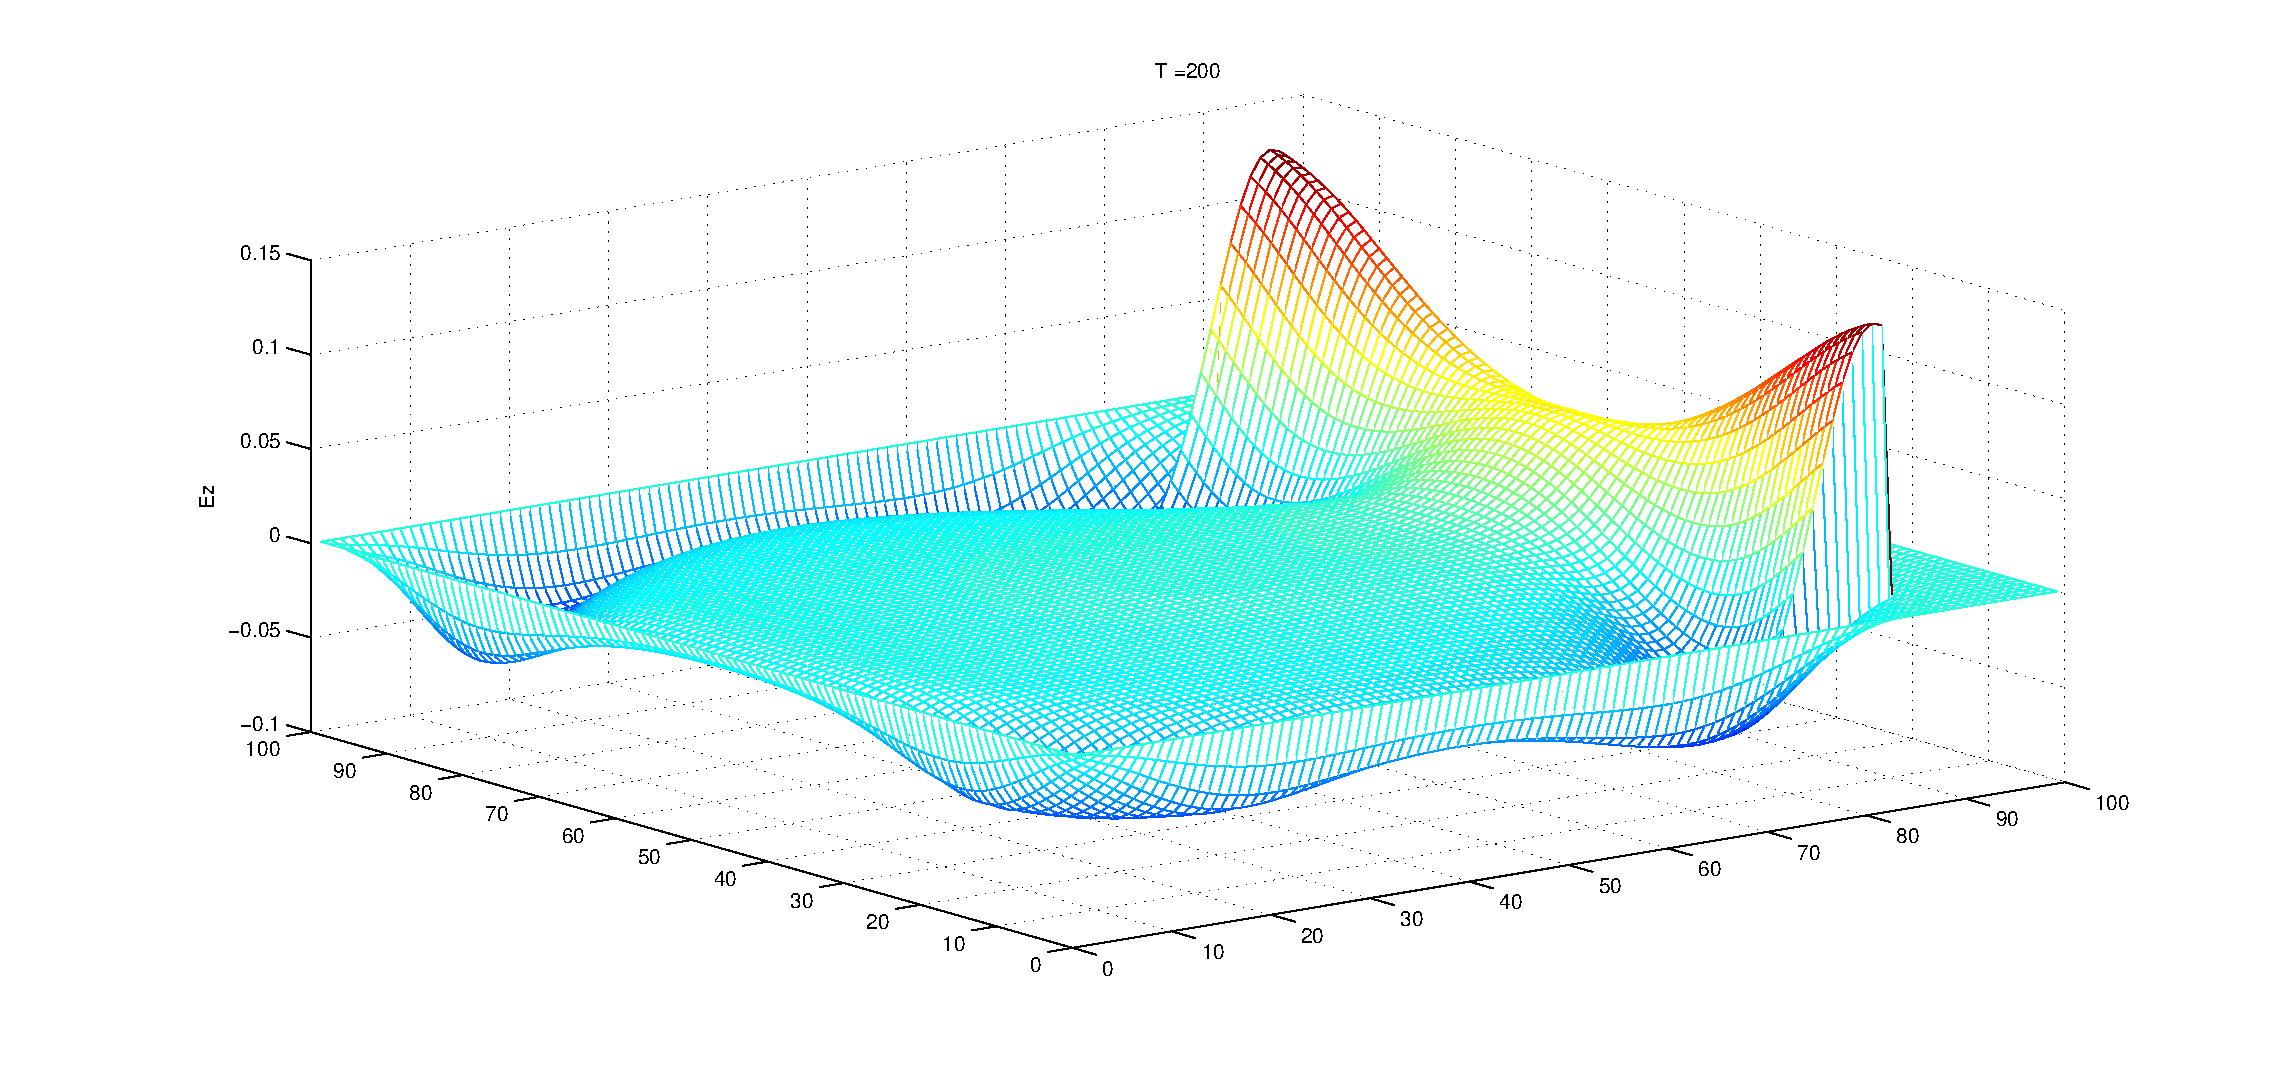
\includegraphics[angle=270,
    width=0.8\textwidth]{ez.200.eps}
\caption{$E_z$ when T = 200.}
\label{pic:ez200}
\end{figure}








\end{document}

